% ======================================================================================== %
\section{Experimental Results}\label{sec:experiment}
% ======================================================================================== %


% ======================================================================================== %
\subsection{Setup}\label{ssec:setup}
% ======================================================================================== %

We train our ASR models on the LibriSpeech-960 dataset~\cite{librispeech}.
For both phoneme classification and speech recognition experiments, we employ 80-dimensional log-Mel filterbank features as the input, extracted from a 25ms window with a 10ms stride.
We employ 36 phoneme classes (including `silence') for the phoneme classification as in~\cite{understanding}.
For speech recognition, the subword vocabulary size is set to 128, built by SentencePiece~\cite{sentencepiece} on the training data transcripts.

We choose the Conformer-M~\cite{conformer} as our baseline and train the model with CTC~\cite{ctc} loss.
The baseline Conformer-M consists of 16 Conformer layers with RPE.
We follow the training details from the previous work~\cite{understanding} for ASR.
For the phoneme classification task, we stack 4 Conformer layers with the hidden dimension of 256.
When replacing SA with phSA, we only modify the self-attention block inside the Conformer layer and preserve other blocks such as convolutional and feed-forward blocks.
We set the learning rate to $1.56\text{e-3}$ and weight decay to $1\text{e-4}$ for the phoneme classification.


% ======================================================================================== %
\subsection{Phoneme Classification}\label{ssec:phoneme}
% ======================================================================================== %

To evaluate the phonetic feature extraction performance, we train the models for phoneme classification.
Table~\ref{tab:per} compares the vanilla SA (M2), phSA (M5), and other variants.
M2 is the original dot-product, and M1 is the same version without bias parameter that only focus on similarity-based relationships.
M3 is identical to the M2 but differs in the implementation that the parameter $W_K$ is not shared.
M1, M2, and M3 show almost similar accuracy with less then 0.1\% difference.
In contrast, M4 shows a noticeable gain in phoneme classification accuracy compared to M2 and M3.
The proposed phSA (M5) achieves the highest accuracy among the dot-product variants.
The results verify that our architectural modifications, M2$\rightarrow$M4 (Sec.~\ref{ssec:decomposition}) and M4$\rightarrow$M5 (Sec.~\ref{ssec:nonlinear}), each contributes to better phonetic feature extraction.


\begin{table}[t]
    \centering 
    \caption{Word error rate (\%) of different configurations of phonetic self-attention layers.
    The baseline performance (without phSA) is presented in the first row.
    The best results are in bold, and the second best results are underlined.}
    \resizebox{0.88\columnwidth}{!}{
    \begin{tabular}{cc|cccc}
        \toprule
        \multicolumn{2}{c|}{\#Layers} & \multicolumn{2}{c}{\textit{dev-}} & \multicolumn{2}{c}{\textit{test-}} \\
        
        phSA & SA & \textit{clean} & \textit{other} & \textit{clean} & \textit{other} \\
        \midrule
        \midrule
        0    & 16 & 3.10 & 8.23 & 3.25 & 8.21 \\
        % 1    & 15 & 3.12 & 8.17 & 3.36 & 8.13 \\
        4    & 12 & \textbf{2.87} & 8.11 & \underline{3.19} & \textbf{7.88} \\
        6    & 10 & \underline{3.01} & \textbf{7.77} & \textbf{3.15} & \underline{7.93} \\
        8    & 8  & 3.05 & \underline{8.06} & \underline{3.19} & 8.06 \\
        12   & 4  & 3.08 & 8.36 & 3.30 & 8.30 \\
        % 15   & 1  & 3.31 & 8.87 & 3.53 & 9.00 \\
        16   & 0  & 3.58 & 9.55 & 3.81 & 9.51 \\
        \bottomrule
    \end{tabular}
    }
    \vspace{-0.2cm}
    \label{tab:wer}
\end{table}


% ======================================================================================== %
\subsection{Speech Recognition}\label{ssec:asr}
% ======================================================================================== %

Table~\ref{tab:wer} shows the end-to-end speech recognition performance with the proposed phSA.
Compared to the baseline, replacing the vanilla SA to phSA reduces the word error rate (WER) on every data subset, especially for the challenging LibriSpeech \textit{dev-other} and \textit{test-other} datasets.
We empirically show that adopting phSA only for lower layers (under $8\text{-th}$ layer) achieves the best performance.
This observation is aligned with previous analysis~\cite{understanding} that the lower layers more focus on phonetic information than upper layers.
For example, replacing phSA for lower 6 layers decreases the WER from 8.23\% to 7.77\% (5.6\% relative reduction) and 8.21\% to 7.93\% (3.4\% relative reduction) for \textit{dev-other} and \textit{test-other} datasets, respectively.
In contrast, utilizing phSA for 12 layers shows worse performance than the baseline, and using phSA for the entire (16) layers suffers from significant performance degradation.


% ======================================================================================== %
\subsection{Discussion}\label{ssec:discussion}
% ======================================================================================== %

\subsubsection{Speed and Parameter Size}

Although we add several new computation steps for phSA, we observe that the training and inference time does not change much.
The main reason is that the removal of RPE can compensate for the additional cost of phSA, in both latency and parameter size.
For example, the wall-clock training time of the phSA ($2^\text{nd}$ row in Table~\ref{tab:wer}) is about 5\% faster than the baseline ($1^\text{st}$ row) with almost the same number of parameters.
% Using more phSA layers can further reduce the time cost, but the benefit is marginal.


% \subsubsection{Phoneme Classification from Hidden Representation}

% To verify whether the performance improvement of phSA comes from the enhanced ability to extract the important phonetic information, we conduct a phoneme classification experiment using intermediate hidden representations (features) extracted from the trained end-to-end ASR models. 
% Specifically, we train a softmax classifier consisting of a single fully-connected layer.
% We compare the baseline (zero phSA layer), 4 phSA layer, and 8 phSA layer models presented in $1^\text{st}, 2^\text{nd}$, and $3^\text{rd}$ rows in Table~\ref{tab:wer}.
% Figure~\ref{fig:prelu} shows the phoneme classification accuracy of different layers' features.
% We observe that there is a consistent accuracy gap between the three models, where the model with 8 phSA layers achieves the highest accuracy.
% The result implies that phSA can be more suitable in phonetic feature extraction than the original SA.


\begin{table}[t]
    \centering
    \caption{Effect of similarity-based (S) and content-based (C) attention by removing each component. 
    Entropy (mean $\pm$ std) of phSA attention maps and word error rate (\%) are reported.}
    \resizebox{0.96\columnwidth}{!}{
    \begin{tabular}{cc|cll}
        \toprule
        % \multirow{2}{*}{S} & \multirow{2}{*}{C} & \multirow{2}{*}{Entropy} & \multicolumn{2}{c}{\textit{test-}} \\
        % & & & \textit{clean} & \textit{other} \\
        S & C & Entropy & \textit{dev-other} & \textit{test-other} \\
        \midrule
        \midrule
        \cmark & \cmark & 1.91 $\pm$ 0.12 & 7.77         & 7.93        \\
        \cmark &        & 2.02 $\pm$ 0.14 & 8.16 (+0.39) & 8.54 (+0.61) \\
               & \cmark & 2.39 $\pm$ 0.04 & 9.20 (+1.43) & 9.35 (+1.42) \\
        \bottomrule
    \end{tabular}
    }
    \label{tab:ablation}
    \vspace{-0.2cm}
\end{table}


\subsubsection{Comparison of Similarity and Content}\label{sssec:comparison}

To understand the relative importance between similarity-based and content-based attention, we evaluate the recognition performance without each component.
Table~\ref{tab:ablation} presents the word error rate of the model using only similarity-related or content-related computation.
Specifically, we fix the parameters of the converged model with 6 phSA layers and discard either term of the phSA dot product (Eq.~\eqref{eq:phsa}).
Removing similarity-based attention (bottom row of Table~\ref{tab:ablation}) degrades the performance more than removing content-based one (top row of Table~\ref{tab:ablation}), which implies that the phonetic features extracted from similarity are more important than content-based attention; however, both are indispensable for speech recognition.

In addition, we calculate the average per-head entropy of attention probability for two settings and observe the meaningful difference.
Similarity-based attention probabilities are more concentrated (lower entropy) and content-based attention probabilities are more distributed (higher entropy).
In other words, the similarity-based term emphasizes the difference while the content-based term enhances the uniformness.
We believe that the proposed phSA encourages two terms to be specialized for different attention patterns.


\subsubsection{PReLU Negative Slope}

The range of PReLU negative slopes is very different for similarity-based and content-based terms after training.
Figure~\ref{fig:prelu} shows the negative slopes $\alpha_{s,c}$ of each attention head.
For similarity-based ones, most of $\alpha_s$ parameters are trained to become much larger than 1, implying that the negative correlation values are aggressively ignored and therefore produce a concentrated probability distribution.
On the other hand, $\alpha_c$ parameters for content-based ones are trained to be smaller than 1, decreasing the difference between negative results.
The combination of large $\alpha_s$ and small $\alpha_c$ is connected to different characteristics discussed in Sec.~\ref{sssec:comparison}.


\begin{figure}[t]
    \centering
    \resizebox{1.0\columnwidth}{!}{
    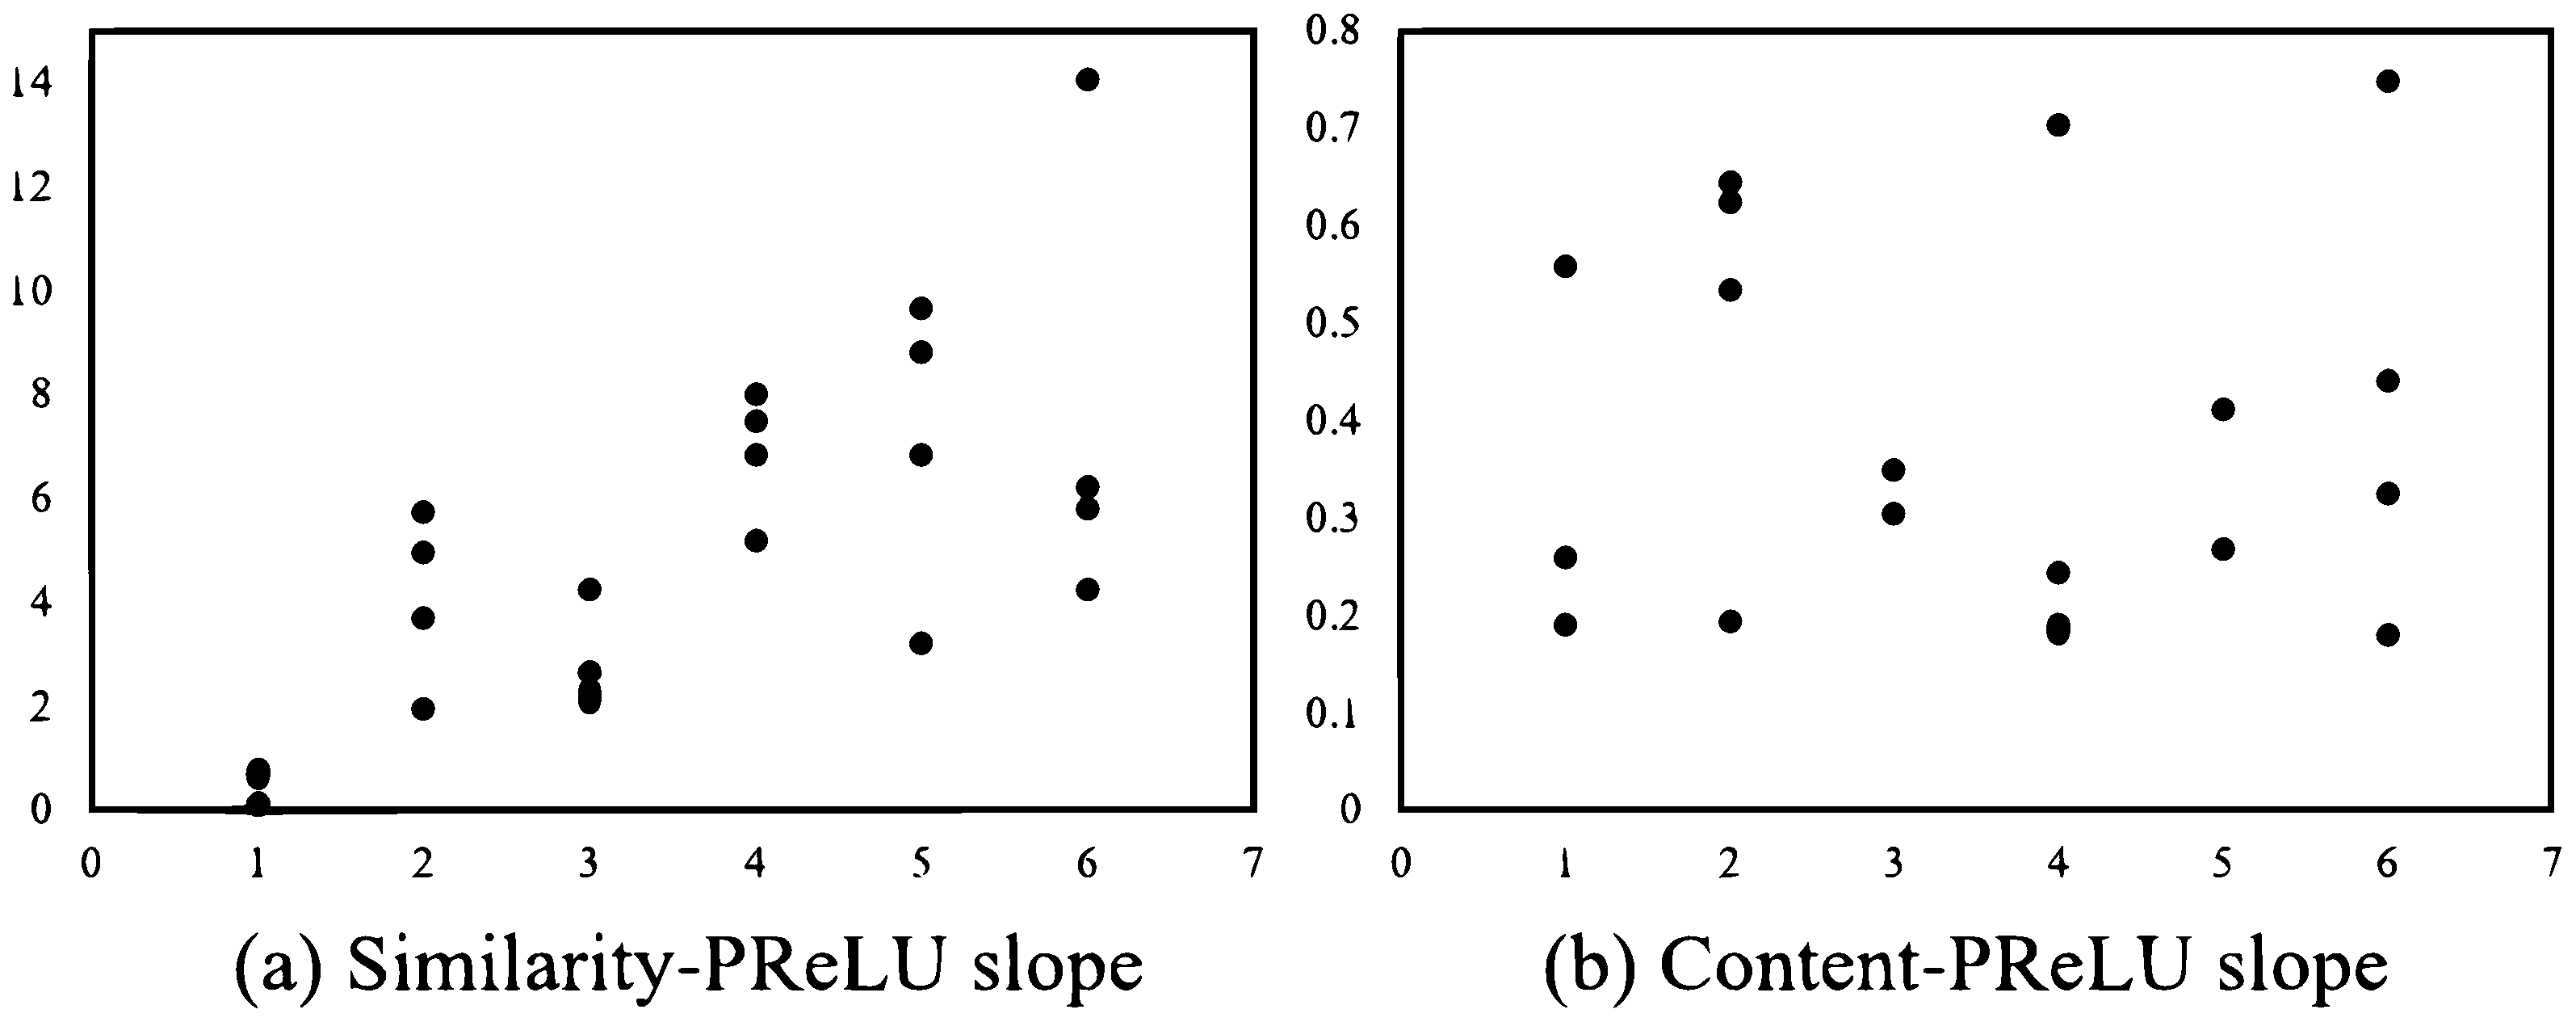
\includegraphics{figure/prelu6.eps}}
    \caption{PReLU negative slopes ($\alpha_s$ and $\alpha_c$) of the phSA after training.
    Four dots in each layer indicates PReLU parameters in four attention heads.
    $x$-axis indicates the layer index.
    Note that the range of $y$-axis is very different, $(0\sim 14)$ for (a) and $(0\sim 0.8)$ for (b).}
    \label{fig:prelu}
    \vspace{0.2cm}
\end{figure}

